\section{Proposta}
\label{proposta}

O terreno geral � dividido em terrenos menores (chamados \emph{patchs}), como mostra o \emph{grid} da Figura \ref{fig:resultados:grid}. Dessa forma, apenas \emph{patchs} de interesse do usu�rio (que est�o mais pr�ximos, por exemplo) precisar�o ser gerados.

\begin{figure}[h]
	\center{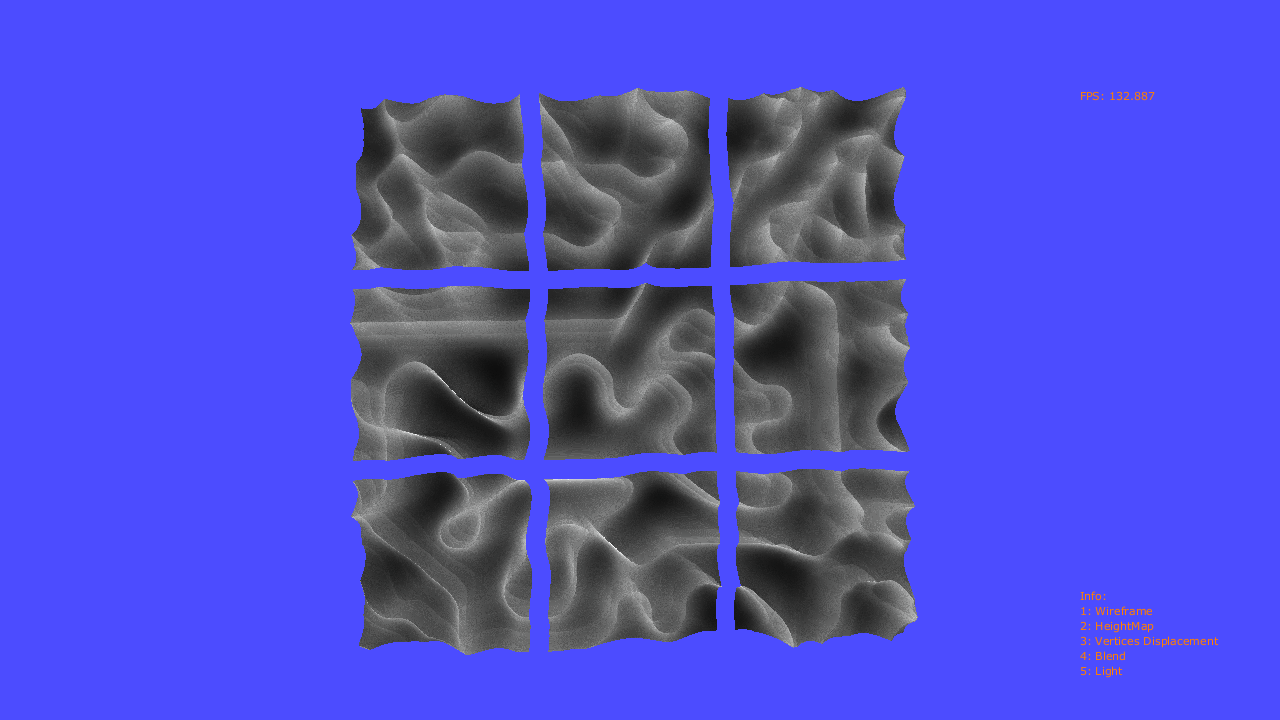
\includegraphics[width=0.6\linewidth]{img/caps/grid.png}}
	\caption{\label{fig:resultados:grid} \emph{Patchs} exibidos em um \emph{grid}.}
\end{figure}

Considerando o usu�rio inicialmente localizado no \emph{patch} central, ao mover-se para um \emph{patch} vizinho, o sistema ir� requisitar a gera�a� de novos \emph{patchs}, vizinhos a aqueles que est�o na borda do grid. O n�mero de vizinhos gerados, bem como a quantidade de vizinhos do \emph{patch} central s�o vari�veis do sistema, podendo ser adaptadas, pelo usu�rio, de acordo com o poder de processamento de sua m�quina.

Para garantir uma visualiza��o fluida do terreno, minimizando as interrup��es com a gera��o, o sistema proposto decide qual arquitetura (GPU ou CPU) ser� utilizada na gera��o dos \emph{patchs}. Considerando \textbf{n} a porcentagem de \emph{patchs} gerados na GPU e \textbf{1 - n} a porcentagem gerado na CPU, no in�cio do sistema, teremos que \textbf{n = m = 0.5}. O aumento da carga para determinada arquitetura ser� decidida ao longo da execu��o do jogo, considerando um hist�rico de frames por segundo.


Tal m�trica foi escolhida pelas seguintes raz�es:

\begin{itemize}
	\item Obter um FPS mais fluido durante a navega��o � um dos principais objetivos deste trabalho.
	\item A mesuriza��o do tempo gasto com trabalho relacionado � parte gr�fica utilizando OpenGL n�o � algo dispon�vel em GPUs. A extens�o \textbf{GL\_EXT\_timer\_query} \cite{timerQuery}, por exemplo, s� est� dispon�vel em placas NVidia, algo que anularia a possibilidade da execu��o deste trabalho em placas ATI.
\end{itemize}

